% Template for PLoS
% Version 1.0 January 2009
%
% To compile to pdf, run:
% latex plos.template
% bibtex plos.template
% latex plos.template
% latex plos.template
% dvipdf plos.template

% TO DELETE
\newcommand{\mike}[1]{\textsf{\emph{\textbf{\textcolor{red}{#1}}}}} 
\newcommand{\dean}[1]{\textsf{\emph{\textbf{\textcolor{green}{#1}}}}} 
\newcommand{\parham}[1]{\textsf{\emph{\textbf{\textcolor{blue}{#1}}}}} 
\newcommand{\ken}[1]{\textsf{\emph{\textbf{\textcolor{magenta}{#1}}}}} 

 % \documentclass[twocolumn,10pt]{article}						%<-use this for checking equation length
 \documentclass[10pt]{article}

% amsmath package, useful for mathematical formulas
\usepackage{amsmath}
% amssymb package, useful for mathematical symbols
\usepackage{amssymb}

% graphicx package, useful for including eps and pdf graphics
% include graphics with the command \includegraphics
\usepackage{graphicx}

% cite package, to clean up citations in the main text. Do not remove.
\usepackage{cite}

\usepackage{color} 

% Use doublespacing - comment out for single spacing
%\usepackage{setspace} 
%\doublespacing

%Set the section counter to one
\setcounter{section}{1}

% Text layout
\topmargin 0.0cm
\oddsidemargin 0.5cm
\evensidemargin 0.5cm
\textwidth 16cm 
\textheight 21cm

% Bold the 'Figure #' in the caption and separate it with a period
% Captions will be left justified
\usepackage[labelfont=bf,labelsep=period,justification=raggedright]{caption}

% Use the PLoS provided bibtex style
\bibliographystyle{plos2009}

% Remove brackets from numbering in List of References
\makeatletter
\renewcommand{\@biblabel}[1]{\quad#1.}
\makeatother


% Leave date blank
% \date{}

\pagestyle{myheadings}
%% ** EDIT HERE **


%% ** EDIT HERE **
%% PLEASE INCLUDE ALL MACROS BELOW
% \usepackage{anysize} 									%<-use this for checking equation length
% \marginsize {1.7cm}{1.5cm}{0.3cm}{0.8cm} 				%<-use this for checking equation length
% \setlength{\columnsep}{0.5cm}							%<-use this for checking equation length
%% END MACROS SECTION

\begin{document}
% Title must be 150 characters or less
\begin{flushleft}
{\Large
\textbf{A Data-Driven Framework for Neural Field Modelling}
}
% Insert Author names, affiliations and corresponding author email.
\\
Dean R. Freestone$^{1,2,3,\ast}$, 
Parham Aram$^{4}$, 
Michael Dewar$^{3,5}$,
Kenneth Scerri$^{6}$,
David B. Grayden$^{1,2}$,
Visakan Kadirkamanathan$^{4}$
\\
\bf{1} Department of Electrical and Electronic Engineering, University of Melbourne, Melbourne, VIC, Australia
\\
\bf{2} The Bionic Ear Institute, East Melbourne, VIC, Australia
\\
\bf{3} Institute for Adaptive and Neural Computation, University of Edinburgh, Edinburgh, UK
\\
\bf{4} Department of Automatic Control and Systems Engineering, University of Sheffield, Sheffield, UK
\\
\bf{5} Department of Applied Physics and Applied Mathematics, Columbia University, New York, NY, USA
\\
\bf{6} Department of Systems and Control Engineering, University of Malta, Msida, MSD, Malta
\\
$\ast$ E-mail: dfreestone@bionicear.org
\end{flushleft}

% Please keep the abstract between 250 and 300 words
\section*{Abstract}
This paper presents a framework for creating neural field models from patient-specific or experimental electrophysiological data. The Wilson and Cowan or Amari style neural field equations are used to form a parametric model, where the parameters are estimated from data. To illustrate the estimation framework, data is generated using the neural field equations incorporating modelled sensors, so a comparison can be made between estimated and true parameters. To facilitate state and parameter estimation, we introduce a method to reduce the continuum neural field model, using a basis function decomposition, forming a finite-dimensional state-space model. Spatial frequency analysis methods are introduced that systematically specify the basis function configuration required to capture the dominant characteristics of the neural field. The estimation procedure consists of a two-stage iterative algorithm incorporating the unscented Rauch-Tung-Striebel smoother for state estimation and a least squares algorithm for parameter estimation. The results show that it is theoretically possible to reconstruct the neural field and estimate intracortical connectivity and synaptic dynamics with the proposed framework. The results also illustrate the loss of high spatial frequency information as the cost incurred by the model reduction procedure. This framework provides a link between neurophysiological data and theoretical neural field models. This link may lead to greater understanding of cortical dynamics at the mesoscopic and macroscopic scales where diseases such as epilepsy are manifested.

% Please keep the Author Summary between 150 and 200 words
% Use first person. PLoS ONE authors please skip this step. 
% Author Summary not valid for PLoS ONE submissions.   
\section*{Author Summary}
With recent advances in medical imaging techniques and computing power, we are entering a new age of neuroscientific research, where patient-specific information and experimental data is becoming incredibly detailed. In order to make the best use of this information, data-driven mathematical models should be formed. This is particularly poignant where considering poorly understood complex systems such as the large-scale dynamics of the human brain. There currently exists a library of mathematical models describing large-scale brain dynamics, providing a theoretical explanation of interesting phenomena associated with various cognitive states and diseases. In this paper, we have created a framework for creating a data-driven mathematical model, forming a bridge between theory and electrophysiological data. Within this framework, we propose rules for designing experiments and we derive the mathematical formula to create the model. To demonstrate the utility of this framework, we provide an example using synthetic data that shows a comparison between true and estimated model characteristics. The ability to create patient-specific models of large-scale brain dynamics has the potential to revolutionise the treatment of diseases such as epilepsy, where techniques from engineering may be used to prevent abnormal neural oscillations.

\section*{Introduction}
Generating physiologically plausible neural field models is of great importance for studying brain dynamics at the mesoscopic and macroscopic scale. While our understanding of the function of neurons is well developed, the overall behaviour of the brain's mesoscopic and macroscopic scale dynamics remains largely theoretical. Understanding the brain at this level is extremely important since it is at this scale that pathologies such as epilepsy, Parkinson's disease and schizophrenia are manifested. 

Mathematical neural field models provide insights into the underlying physics and dynamics of electroencephalography (EEG) and magnetoencephalography (MEG) (see~\cite{Deco2008,David2003} for recent reviews). These models have demonstrated possible mechanisms for the genesis of neural rhythms (such as the alpha and gamma rhythms) \cite{Liley1999,RENNIE2000}, epileptic seizure generation \cite{DaSilva2003,Suffczynski2004,Wendling2005} and insights into other pathologies \cite{Moran2008,Schiff2009} that would be difficult to gain from experimental data alone. 

Unfortunately, the use of these models in the clinic has been limited, since they are constructed for ``general'' brain dynamics whereas pathologies almost always have unique underlying patient-specific causes. Patient-specific data from electrophysiological recordings is readily available in the clinical setting, particularly from epilepsy surgery patients, suggesting an opportunity to make the patient-specific link to models of cortical dynamics. Furthermore, recent technological advances have driven an increased level of sophistication in recording techniques, with dramatic increases in spatial and temporal sampling~\cite{Brinkmann2009}. However, the mesoscopic and macroscopic neural dynamic state is not directly observable in neurophysiological data, making predictions of the underlying physiology inherently difficult.

For models to be clinically viable, they must be patient-specific. A possible approach to achieve this would be to fit a general continuum neural field model, like the Wilson and Cowan (WC)~\cite{Wilson1973} or Amari~\cite{Amari1977} models or a neural mass model like the Jansen and Ritt model~\cite{Jansen1995} to patient-specific data. Fitting the neural models to individuals is a highly non-trivial task and, until very recently, has not been reported in the literature. 

An estimation framework for neural mass models known as dynamical causal modelling (DCM) \cite{David2003,David2006} has recently been proposed for studying evoked potential dynamics. Via a Bayesian inference scheme, DCM estimates the long range (cortico-cortical) connectivity structure between the specific isolated brain regions that best explains a given data set using the Jansen and Ritt equations~\cite{Jansen1995}. Another recent publication describing a parameter estimation method with a neural field model used an unscented Kalman filter with modified WC neural field equations~\cite{schiff2008kalman}. This work takes a system theoretic approach to the neural estimation problem, successfully demonstrating that it is possible to perform state estimation on spatiotemporal neural fields. This marks the first step in what has the potential to revolutionise the treatment of many neurological diseases where therapeutic electrical stimulation is viable.

We present an extension to the work of Schiff and Sauer~\cite{schiff2008kalman} by establishing a framework for estimating the state of the WC equations for larger scale (more space) systems via a systematic model reduction procedure. In addition, a method is presented for estimating the connectivity structure and the synaptic dynamics. Until now, model-based estimation of local intracortical connectivity has not been reported in the literature (to the best of the authors' knowledge). Our study builds on recent work which shows that it is possible to estimate local coupling of spatiotemporal systems using techniques from control systems theory and machine learning~\cite{Dewar2009}. The key development of this previous work was to represent a spatiotemporal system as a standard state-space model, with the number of states independent of the number of observations (recording electrodes in this case). In addition, the appropriate model selection tools have been developed~\cite{Scerri2009} allowing for the application of the technique to neural fields. 

Modelling the neural dynamics within this framework has a distinct advantage over the more standard multivariate auto-regressive (MVAR) models: the number of parameters to define the spatial connectivity is considerably smaller than the number of AR coefficients typically required to achieve the required model complexity. 

In this paper, we demonstrate for the first time how intracortical connectivity can be inferred from data, based on a variant of the WC neural field model~\cite{Wilson1973}. This work provides a fundamental link between the theoretical advances in neural field modelling and electrophysiological data. The paper proceeds by first deriving the continuum neural field equations. Then a finite-dimensional neural field model is derived. The model is reduced by approximating the neural field using a set of continuous basis functions, weighted by a finite dimensional state vector. The next section establishes conditions using spatial frequency analysis for both sensor and basis function spacing and width, such that the dominant dynamics of the neural field can be represented by the reduced model. The state and parameter estimation procedure is described in the following section. The results for the spatial frequency analysis and parameter estimation are then presented. Finally, the implications and limitations of this framework are discussed along with planned future developments.

% You may title this section "Methods" or "Models". 
% "Models" is not a valid title for PLoS ONE authors. However, PLoS ONE
% authors may use "Analysis" 
\section*{Methods}

\subsection*{Neural Field Model}\label{NeuralModelSection} 
Neural field models relate mean firing rates of pre-synaptic neural populations to mean post-synaptic membrane potentials. They are popular as they are parsimonious yet have a strong link with the underlying physiology. Each neural population represents a functional cortical processing unit, such as a column. The columnar organisation of the cortex is continuous, where pyramidal cells are members of many columns. In general, cortical structure can be modelled in a physiologically plausible manner as being locally homogeneous (in short range intracortical connectivity) and heterogeneous (in long range cortico-cortical and corticothalamic connectivity)~\cite{Jirsa2009,Qubbaj2007}. In certain regions of the cortex, each column is thought to be connected locally via symmetric short range local excitation with surround inhibition \cite{Braitenberg1998}. For example, this structural organisation is most studied in the visual system, where the surrounding inhibition effectively tunes a cortical column to a particular receptive visual field~\cite{Sullivan2006}. Neural field models are descriptive of a range of neurodynamics of the cortex such as evoked potentials, visual hallucinations and epileptic behaviour~\cite{David2003,Bressloff2001,Breakspear2006}. Field models are also capable of generating complex spatial patterns of activity such as Turing patterns, spirals and travelling oscillations~\cite{Amari1977,Coombes2005,Coombes2007}.

\subsection*{Derivation of the Integro-Difference Equation Representation}
The model relates the average number of action potentials $g(\mathbf{r},t)$ arriving at position $\mathbf{r}$ to the local post-synaptic membrane voltage $v(\mathbf{r},t)$. Note, Table~\ref{tab:Notation} provides a description of the notation used in this study. The post-synaptic potentials generated at a neuronal population at location $\mathbf{r}$ by action potentials arriving from all other connected populations at locations $\mathbf{r}'$ is described by 
\begin{equation}
	\label{SpikesToPotential} v\left( {\mathbf{r},t} \right) = \int_{ - \infty }^t {h\left( {t - t'} \right)g\left( {\mathbf{r},t'} \right)dt'}. 
\end{equation}
The post-synaptic response kernel $h(t)$ is described by 
\begin{equation}
	\label{SynapticRespKernel} h(t) = \eta(t)\exp{\left(-\zeta t\right)}, 
\end{equation}
where $\zeta=\tau^{-1}$, $\tau$ is the synaptic time constant and $\eta(t)$ is the Heaviside step function. Non-local interactions between cortical populations are described by 
\begin{equation}
	\label{RateBasedInteractions} g\left( \mathbf{r},t \right) = \int_\Omega {w\left( \mathbf{r},\mathbf{r}' \right)f\left( v\left( \mathbf{r}',t \right) \right)\textrm{d}\mathbf{r}'}, 
\end{equation}
where $f(\cdot)$ is the firing rate function, $w(\cdot)$ is the spatial connectivity kernel and $\Omega$ is the spatial domain representing a cortical sheet or surface. The connectivity kernel is typically a ``Mexican hat'' function, which describes local excitation and surround inhibition. An example of the connectivity kernel is shown in Figure~\ref{fig:2d_kernel}. To demonstrate flexibility in the estimation algorithm, a third component of the kernel is introduced describing weak longer-range excitation. The exact shape of this kernel is assumed to vary across patients, and hence needs to be inferred from data.

The firing rate of the presynaptic neurons is related to the postsynaptic membrane potential by the sigmoidal activation function 
\begin{equation}
	\label{ActivationFunction} f\left( v\left( \mathbf{r}', t \right) \right) = \frac{f_{max}}{1 + \exp \left( \varsigma \left( v_0 - v\left(\mathbf{r}',t\right) \right) \right)}. 
\end{equation}
The parameters $f_{max}$ and $v_0$ describe the maximum firing rate and firing threshold of the neural populations respectively. The parameter $\varsigma$ governs the slope of the sigmoid. By substituting equation~\ref{RateBasedInteractions} into equation~\ref{SpikesToPotential} we get the spatiotemporal model 
\begin{equation}
	\label{FullDoubleIntModel} v\left(\mathbf{r},t\right) =
	\int_{-\infty}^t 
	h\left(t - t'\right) \int_\Omega
	w\left(\mathbf{r},\mathbf{r}'\right) 
	f\left( v\left( \mathbf{r}',t' \right)\right)
	\textrm{d}\mathbf{r}'dt'.
\end{equation}
To arrive at the final form of the model, we shall express the synaptic response kernel as a Green's function 
\begin{equation}
	\label{GreensFuncDef} Dh\left( t \right) = \delta \left( t \right), 
\end{equation}
where $D=\frac{d}{dt} + \zeta$ is a temporal differential operator and $\delta(t)$ is the Dirac-delta function giving 
\begin{equation}
	\label{FinalFormContinuous} 
	\frac{dv\left( \mathbf{r},t \right)}{dt} + \zeta v\left( \mathbf{r},t \right) = \int_\Omega {w\left( \mathbf{r},\mathbf{r}' \right)f\left( {v\left( \mathbf{r}',t \right)} \right)\textrm{d}\mathbf{r}'}. 
\end{equation}
To arrive at the integro-difference equation (IDE) form of the model, we discretise time using a first-order Euler method (see the S1 for derivation) giving 
\begin{equation}
	\label{DiscreteTimeModel} 
	v_{t+T_s}\left(\mathbf{r}\right) = 
	\xi v_t\left(\mathbf{r}\right) + 
	T_s \int_\Omega { 
	    w\left(\mathbf{r},\mathbf{r}'\right)
	    f\left(v_t\left(\mathbf{r}'\right)\right) 
	\textrm{d}\mathbf{r}'} 
	+ e_t\left(\mathbf{r}\right), 
\end{equation}
where $T_s$ is the time step, $\xi = 1-T_s\zeta $ and $e_t(\mathbf{r})$ is an $i.i.d.$ disturbance such that $e_t(\mathbf{r})\sim\mathcal{GP}(\mathbf 0,\gamma(\mathbf{r}-\mathbf{r}'))$. Here $\mathcal{GP}(\mathbf 0,\gamma(\mathbf{r}-\mathbf{r}'))$ denotes a zero mean spatial Gaussian process with covariance function $\gamma(\mathbf{r}-\mathbf{r}')$~\cite{Rasmussen2005}. This term is added to account for model uncertainty and unmodelled inputs. To simplify the notation, the index of the future time sample, $t+T_s$, shall be referred to as $t+1$ throughout the rest of the paper. 

The mapping between the membrane voltage and the electrophysiological data is modelled using the observation function that incorporates sensors with a spatial extent by
\begin{equation}
    \label{eq:ObservationEquation}
	\mathbf{y}_t =
	\int_{\Omega}{
	    m\left(\mathbf{r}_n-\mathbf{r}'\right)v_t\left(\mathbf{r}'\right)
	\textrm{d}\mathbf{r}'} + 
	\boldsymbol{\varepsilon}_t, 
\end{equation}
where $\mathbf{r}_n$ defines the location of the sensors in the field, $n=1,...,N$ indexes the sensors and $\boldsymbol{\varepsilon}_t \sim \mathcal{N}\left(0,\boldsymbol{\Sigma}_{\varepsilon}\right)$. $\mathcal{N}\left(0,\boldsymbol{\Sigma}_{\varepsilon}\right)$ denotes the multivariate normal distribution with mean zero and covariance matrix $\boldsymbol{\Sigma}_{\varepsilon}$. The output kernel $m(\mathbf{r}-\mathbf{r}')$ governs the sensor pick-up geometry and is defined by 
\begin{equation}
	m\left(\mathbf{r}-\mathbf{r}'\right) = \exp{\left(-\frac{(\mathbf{r}-\mathbf{r}')^\top(\mathbf{r}-\mathbf{r}')}{\sigma_m^2}\right)},
\end{equation}
where $\sigma_m$ sets the sensor width.

\subsection*{Derivation of Finite Dimensional State-Space Model}\label{Sect:ReducedModelDerivation}
In order to implement standard estimation techniques, we use a decomposition of the field using a set of Gaussian basis functions that are defined by
\begin{equation}\label{eq:FieldBasisFunction}
	\boldsymbol\phi\left(\mathbf{r}-\mathbf{r}'\right) =
\exp{\left(-\frac{(\mathbf{r}-\mathbf{r}')^\top(\mathbf{r}-\mathbf{r}')}{\sigma_{\phi}^2}\right)}. 
\end{equation}
Decomposition allows a continuous field to be represented by a finite-dimensional state vector. This facilitates application of standard nonlinear state estimation methods such as the unscented Kalman filter. The field decomposition is described by 
\begin{equation}
	\label{DefFieldDecomp} v_t\left(\mathbf{r}\right) \approx \boldsymbol{\phi}^{\top}\left(\mathbf{r}\right) \mathbf{x}_t, 
\end{equation}
where $\mathbf{\boldsymbol{\phi}}(\mathbf{r})$ is a vector of Gaussian basis functions that are scaled by the state vector, $\mathbf{x}_t$. An example of a one-dimensional field decomposition is given in Figure~\ref{fig:FieldDecomposition}.%The choice of Gaussian basis functions can be justified by the existence of the so called bump solutions for this class of model, which have a Gaussian shape~\cite{Coombes2005}.

The width and positioning of the basis functions can be determined by spectral analysis (explained in detail in the following section). The connectivity kernel can also be decomposed as 
\begin{equation}\label{DefKernelDecomp}
	 w\left(\mathbf{r},\mathbf{r}'\right) =\boldsymbol{\psi}^\top\left(\mathbf{r},\mathbf{r}'\right) \boldsymbol{\theta},
\end{equation}
where $\boldsymbol{\psi}(\mathbf{r},\mathbf{r}')$ is a vector of Gaussian basis functions and $\boldsymbol{\theta}$ is a vector of scaling parameters. By assuming a Gaussian isotropic connectivity structure, the kernel basis functions can be written as $\boldsymbol{\psi}(\mathbf{r}-\mathbf{r}')$. We will assume that we know the parametric form of the connectivity basis functions, where the scaling parameters $\boldsymbol{\theta}$ are unknown. Each connectivity basis function can, individually, be considered a layer in the Wilson and Cowan model. Typically, the Mexican hat connectivity kernel is comprised of two basis functions representing local excitation and surround inhibition. To demonstrate the flexibility of the estimation framework, a third basis function is incorporated, corresponding to weaker mid-range excitation. Making substitutions of equations~\ref{DefFieldDecomp} and~\ref{DefKernelDecomp} into~\ref{DiscreteTimeModel} we get 
\begin{equation}
	\label{reduced continuous model}\boldsymbol{\phi}^{\top}(\mathbf{r})\mathbf{x}_{t+1}= T_s\int_\Omega{f(\boldsymbol{\phi}^{\top}(\mathbf{r}')\mathbf{x}_t )\boldsymbol{\psi}^{\top}(\mathbf{r}-\mathbf{r}')\textrm{d}\mathbf{r}'}\boldsymbol{\theta}
	+ \xi\boldsymbol{\phi}^{\top}(\mathbf{r})x_t + e_t(\mathbf{r}). 
\end{equation}
Next we multiply equation~\ref{reduced continuous model} by $\boldsymbol{\phi}(\mathbf{r})$ and integrate over the spatial domain $\Omega$ to get 
\begin{equation}
    \begin{split}
	\label{StartofReduction}
	\lefteqn{ \int_\Omega {\boldsymbol{\phi} \left(\mathbf{r}\right)\boldsymbol{\phi}^{\top}\left(\mathbf{r}\right) \textrm{d}\mathbf{r}} \mathbf{x}_{t+1}=} \\
 &T_s \int_\Omega {\boldsymbol{\phi} (\mathbf{r}) \int_\Omega {\boldsymbol{\psi}^{\top} (\mathbf{r}-\mathbf{r}') f(\boldsymbol{\phi}^{\top}(\mathbf{r}') \mathbf{x}_t ) \textrm{d}\mathbf{r}'}\textrm{d}\mathbf{r}}\boldsymbol{\theta}  + \xi\int_\Omega {\boldsymbol{\phi}(\mathbf{r})\boldsymbol{\phi}^{\top}(\mathbf{r})\textrm{d}\mathbf{r}} \mathbf{x}_t+
\int_\Omega{\boldsymbol{\phi} (\mathbf{r}) e_t(\mathbf{r})\textrm{d}\mathbf{r}}. 
\end{split}
\end{equation}
Now defining the matrix
\begin{equation}\label{eq:DefGamma}
	\boldsymbol{\Gamma} \triangleq \int_\Omega {\boldsymbol{\phi} \left(\mathbf{r}\right)\boldsymbol{\phi} ^{\top}\left(\mathbf{r}\right)\textrm{d}\mathbf{r}}, 
\end{equation}
and substituting this into equation~\ref{StartofReduction} and cross-multiplying by $\boldsymbol{\Gamma}^{-1}$ gives 
\begin{equation}
    \label{eq:ReducedForm}
    \begin{split}
	 \mathbf{x}_{t+1} = T_s\boldsymbol{\Gamma}^{-1}
	 \int_\Omega \boldsymbol{\phi}(\mathbf{r}) 
	 \int_\Omega \boldsymbol{\psi}^{\top} (\mathbf{r}-\mathbf{r}')f(\boldsymbol{\phi}^{\top}(\mathbf{r}')\mathbf{x}_t) \textrm{d}\mathbf{r}' \textrm{d}\mathbf{r} \boldsymbol{\theta}  
	 + \xi\mathbf{x}_t + \boldsymbol{\Gamma}^{-1} \int_\Omega{\boldsymbol{\phi}(\mathbf{r}) e_t(\mathbf{r})\textrm{d}\mathbf{r}}.
	 \end{split}
\end{equation}
The analytic derivation of the inner product of \emph{n}-dimensional Gaussians, which was used for calculating $\Gamma$, is provided in the Supporting Information, S1. Equation~\ref{eq:ReducedForm} can be simplified by exploiting the isotropy of the kernel and, hence, the basis functions used to represent it where

\begin{equation}
	\boldsymbol{\psi} (\mathbf{r}-\mathbf{r}') = \boldsymbol{\psi} (\mathbf{r}'-\mathbf{r}).
\end{equation}
To make the simplification, we first define
\begin{equation}\label{eq:DefPsi}
	\boldsymbol{\Psi}(\mathbf{r}') \triangleq T_s\boldsymbol{\Gamma}^{-1}\int_\Omega {\boldsymbol{\phi}(\mathbf{r})\boldsymbol{\psi}^{\top} (\mathbf{r}'-\mathbf{r})\textrm{d}\mathbf{r}},
\end{equation}
which is a constant $L \times n_{\theta}$ matrix that is defined analytically (see the Supporting Information, S1, for analytic convolution of two Gaussians), where $L$ is the number of basis functions (and states) and $n_{\theta}$ is the number of connectivity kernel basis functions. Substituting equation~\ref{eq:DefPsi} into~\ref{eq:ReducedForm} gives
\begin{equation}
	\mathbf{x}_{t+1} = \int_\Omega \boldsymbol{\Psi}(\mathbf{r}') f(\boldsymbol{\phi}^{\top}(\mathbf{r}')\mathbf{x}_t) \textrm{d}\mathbf{r}' \boldsymbol{\theta} + \xi\mathbf{x}_t 
+ \boldsymbol{\Gamma}^{-1} \int_\Omega{\boldsymbol{\phi}(\mathbf{r})e_t(\mathbf{r})\textrm{d}\mathbf{r}}.
\end{equation}
This simplification has transformed the description of the spatial coupling from a convolution of the firing rates with the connectivity kernel, to a convolution of the connectivity kernel basis functions with the field basis functions. This transformation provides a dramatic increase in estimation speed, since the matrix $\boldsymbol\Psi(\mathbf{r}')$ is constant and can be pre-defined analytically. This is of great importance considering the computational demands of the estimation algorithm. 

Now we define the state disturbance as
\begin{equation}\label{eq:Wt} 
	\mathbf{e}_t \triangleq \boldsymbol{\Gamma}^{-1}\int_\Omega {\boldsymbol{\phi} ( \mathbf{r} )e_t( \mathbf{r} )\textrm{d}\mathbf{r}},
\end{equation}
which is a zero mean normally distributed white noise process with covariance (see the Supporting Information, S1, for the derivation)
\begin{equation}
	\boldsymbol\Sigma_e =\mathbf{\Gamma}^{-1}\int_{\Omega}\int_{\Omega}\boldsymbol{\phi}\left(\mathbf r\right) \gamma\left(\mathbf r- \mathbf r' \right)\boldsymbol{\phi}\left(\mathbf r'\right)^{\top}d\mathbf r' d\mathbf r\mathbf{\Gamma}^{- \top}. 
\end{equation}
Under the assumption that the basis function decomposition is accurate, the observation equation of the reduced model is found by substituting equation~\ref{DefFieldDecomp} into~\ref{eq:ObservationEquation} giving
\begin{equation}\label{eq:ReducedObservationEquation}
	\mathbf{y}_t = \int_{\Omega}{m\left(\mathbf{r}_n-\mathbf{r}'\right)\boldsymbol{\phi}^{\top}\left(\mathbf{r'}\right) \mathbf{x}_t\textrm{d}\mathbf{r}'} + \boldsymbol{\varepsilon}_t. 
\end{equation}
The observation equation is linear and can be written in the more compact form
\begin{equation}\label{ObservationEquation} 
	\mathbf{y}_t = \mathbf{C}\mathbf{x}_t + \boldsymbol{\varepsilon}_t,
\end{equation}
where the observation matrix is 
\begin{equation}
	\mathbf{C} = \left[
	\begin{array}{{ccc}} 
		c_{1,1} & \dots & c_{1,L} \\
		\vdots & \ddots & \vdots \\
		c_{N,1} & \dots & c_{N,L} 
	\end{array}
	\right] 
\end{equation}
and 
\begin{equation}
	c_{i,j} = \int_{\Omega}m(\mathbf{r}_i - \mathbf{r}')\boldsymbol{\phi}_j(\mathbf{r}')\textrm{d}\mathbf{r}'. 
\end{equation}
Now we have the final form of the state-space model where
\begin{equation}\label{eq:finalformstatespacemodel}
	\mathbf{x}_{t+1} = Q(\mathbf{x}_t) +\mathbf{e}_t
\end{equation}
\begin{equation} 
	\mathbf{y}_t = \mathbf{C}\mathbf{x}_t + \boldsymbol{\varepsilon}_t
\end{equation}
and 
\begin{equation}\label{eq:QmatrixForSigmapoints}
	Q(\mathbf{x}_t) = \int_\Omega \boldsymbol{\Psi}(\mathbf{r}') f(\boldsymbol{\phi}^{\top}(\mathbf{r}')\mathbf{x}_t) \textrm{d}\mathbf{r}' \boldsymbol{\theta} + \xi\mathbf{x}_t.
\end{equation}

\subsection*{Spectral Analysis}\label{SpectralAnalysisSection} 
Spectral analysis has been used to identify both the number of sensors and the number of basis functions required to reconstruct the neural field from sampled observations~\cite{Sanner1992,Scerri2009}. Based on a two-dimensional extension of Shannon's sampling theorem \cite{Peterson1962}, the spatial bandwidth of the observed field can be used to provide a lower bound on both the number of sensors and the number of basis functions required to capture the dominant spectral characteristics of the neural field.

Let the spectral representation of the post-synaptic membrane voltage field at time $t$ be denoted by $V_t(\boldsymbol{\nu})$. According to Shannon's sampling theorem, the field must be spatially band-limited for an accurate reconstruction using spatially discrete observations. Nevertheless, an approximate reconstruction can be obtained if the field is approximately band-limited with 
\begin{equation}
	V_t(\boldsymbol{\nu}) \approx 0 ~ \ \forall \boldsymbol{\nu} > \boldsymbol{\nu}_c,
\end{equation}
where $\boldsymbol{\nu}_c$ is a cutoff frequency (typically taken as the -3~dB point). Given such a band-limited field, the distance between adjacent sensors, $\Delta_y$, must satisfy 
\begin{equation}
	\label{eq:MinimumSensorDistance} \Delta_y \leq \frac{1}{2\rho_y\boldsymbol{\nu}_{c}}, 
\end{equation}
where $\rho_y \in \mathbb{R} \ge 1$ is an oversampling parameter. This condition must be satisfied to avoid spatial spectral aliasing effects when reconstructing the hidden dynamic field, $v_t(\mathbf{r})$, using the sampled observations, $\mathbf{y}_t$.

In practice, it is difficult to estimate the bandwidth of the cortex using traditional electrophysiological measurements, possibly preventing placement of sensors in accordance to equation~\ref{eq:MinimumSensorDistance}. However, we envisage it may be possible to estimate the spatial bandwidth using other modalities with higher spatial resolution such as fMRI, NIRS or other optical imaging techniques~\cite{Issa2000}. Nevertheless, spectral aliasing can still be avoided by a proper choice of the spatial sampling distance given the sensors' spectral characteristics. The spatial extent of the sensors results in a spectral low-pass action, thus providing spatial anti-aliasing filtering. Such sensors, therefore, can only sense the field up to a known spatial bandwidth, denoted by $\boldsymbol{\nu}_{cy}$. Aliasing can then be avoided by positioning the sensors according to equation~\ref{eq:MinimumSensorDistance}, replacing $\boldsymbol{\nu}_c$ with $\boldsymbol{\nu}_{cy}$.

Although such sensors avoid errors due to aliasing, they attenuate the high spatial frequency variations in the observations. Therefore, any procedure applied to estimate the original field or the underlying connectivity structure from these band-limited observations has the potential to underestimate the high spatial frequency components of both the field and the connectivity kernel. This motivates the use of sensors with wider bandwidths (narrower in space). Nevertheless, this choice would require more sensors in order to satisfy Shannon's sampling theorem for a given spatial region. Therefore, a compromise needs to be found between the bandwidth of the sensor response, the accuracy of the estimation results, the number of sensors and the computational demands of the estimation procedure when designing experiments.

Similar considerations need to be made regarding the representation of the dynamic field, $v_t(\mathbf{r})$, using the basis function decomposition. Again applying Shannon's sampling theorem, the minimum distance between basis functions must satisfy 
\begin{equation}\label{eq:BasisFunctionSeparation}
	\Delta_{\phi} \leq \frac{1}{2\rho_{\phi}\boldsymbol{\nu}_{cy}}
\end{equation}
where $\rho_{\phi} \in \mathbb{R} \ge 1$ is an oversampling parameter to determine the basis function separation. 

The field basis function widths can also be inferred using spectral considerations~\cite{Sanner1992,Scerri2009}. To demonstrate this, we begin with a two-dimensional Gaussian basis function located at the origin, defined as
\begin{equation}\label{eq:BasisFunctionAtOrigin}
 \phi(\mathbf r)=\mathrm{exp}\left({-\frac{1}{\sigma_{\phi}^2} \mathbf r^\top\mathbf r}\right).
\end{equation}
The corresponding Fourier transform is
\begin{equation}\label{eq:GaussianFT}
\boldsymbol\Phi(\boldsymbol \nu)=\left(\frac{1}{\pi\sigma_{\nu}^2}\right)\mathrm{exp}\left(-\frac{1}{\sigma_{\nu}^2}\boldsymbol\nu^\top \boldsymbol\nu\right),
\end{equation}
where 
\begin{equation}\label{eq:GaussianFTWidth}
	\sigma^2_{\nu} = \frac{1}{\pi^2\sigma_{\phi}^2}. 
\end{equation}
To obtain a 3~dB attenuation at $\boldsymbol\nu_{cy}$, the basis function width, $\sigma^2_{\phi}$, should be chosen to be
\begin{equation}\label{eq:WidthCutOffRelationship}
 \sigma^2_{\phi}= \frac{1}{\pi^2\sigma_{\nu_{cy}}^2},
\end{equation}
where
\begin{equation}\label{eq:WidthFrequencyRelationship}
 \sigma^2_{\nu_{cy}}= \frac{2\boldsymbol\nu_{cy}^\top \boldsymbol\nu_{cy}}{\ln2}.
\end{equation}
This ensures that the basis functions can represent the neural field with frequency content up to $\boldsymbol\nu_{cy}$. Derivations for equations~\ref{eq:GaussianFT} and \ref{eq:WidthFrequencyRelationship} are given in the Supporting Information, S1.

Alternatively, the basis function width can be set to provide a desired level of smoothness in the approximated field by reducing the spatial bandwidth. This allows for an approximate representation by a lower order model (fewer basis functions), thus reducing the computational demands of the estimation process. The spatial cut-off frequency of this smoothed field becomes a design choice. To calculate the cut-off frequency imposed by the basis functions, $\boldsymbol{\nu}_{c\phi}$, we rearrange equations~\ref{eq:WidthCutOffRelationship} and \ref{eq:WidthFrequencyRelationship} giving
\begin{equation}\label{eq:CutoffFromBasisFuncWidth}
	\nu_{c\phi}=\frac{1}{\pi\sigma_{\phi}}\sqrt{\frac{\ln2}{2}}.
\end{equation} 

Note that for a spatially homogeneous isotropic field, the basis functions can be placed on a regular grid. Thus, the knowledge of the distance between basis functions can be used to determine the total number of basis functions required to represent a known spatial region.

\subsection*{State and Parameter Estimation}\label{StateAndParameterEstimationSection} In this section, we describe the procedure for estimating the states, $\mathbf{x}_t$, the connectivity kernel parameters, $\boldsymbol \theta$, and the synaptic dynamics, $\xi$. The estimation process is a two part iterative algorithm, consisting of a state estimation step followed by a parameter estimation step. At each iteration, the sequence of estimated state vectors is used to update the parameter set. The resulting parameters are then used when estimating the new state vector sequence for the next iteration. The procedure stops when the parameters converge. The algorithm is initialised using a bounded random state vector sequence, guaranteeing that the initial estimated parameter set forms a stable kernel.

The unscented Rauch-Tung-Striebel smoother (URTSS)~\cite{Sarkka2010} is used for the state estimation. The URTSS incorporates an unscented Kalman filter (UKF)~\cite{Julier1997, Merwe2003} in a forward step to estimate posterior states, $\hat{\mathbf x}_t^{f}$, followed by a backward step to compute the smoothed state estimates, $\hat{\mathbf x}_t^{b}$. The first and second order moments of the predicted state are captured by propagating the so-called sigma points through the state equation. The sigma points, $\mathcal X_i$, are calculated using the unscented transform as follows:
\begin{align}\label{eq:sigmapoints1}
	\mathcal X_{0}&=\bar x \\
	\mathcal X_{i}&=\bar x+\left(\sqrt{( L + \lambda)\mathbf P_x}\right)_i, \quad i=1, \dots, L \\
	\mathcal X_{i}&=\bar x-\left(\sqrt{( L + \lambda)\mathbf P_x}\right)_{i- L}, \quad i= L+1, \dots, 2L 
\end{align}
where $\bar x$ represents either $\hat{\mathbf x}_t^{f}$ or $\hat{\mathbf x}_t^{b}$, $\mathbf{P}_x$ is the corresponding covariance matrix for filtering or smoothing, $\left(\sqrt{( L + \lambda)\mathbf P_x}\right)_i$ is the $i^{th}$ column of the scaled matrix square root of $\mathbf P_x$ and $L$ is the dimension of the state space. The total number of sigma points is $2L+1$. The scaling parameter, $\lambda$, is defined as 
\begin{equation}\label{eq:sigmapoints3}
	\lambda=\alpha^2( L+\kappa) - L, 
\end{equation}
where the constant $\alpha$ determines the spread of the sigma points, $\beta$ incorporates prior knowledge of the distribution of $\mathbf{x}$ and $\kappa$ is an additional scaling parameter (see~\cite{Haykin2001} for more details). 

The sigma vectors are propagated through the system equations and weighted to form the predicted mean and covariance. The weights are calculated by 
\begin{align}
	\mathbf W_0^{(m)}&=\frac{\lambda}{ L+\lambda} \\
	\mathbf W_0^{(c)}&=\frac{\lambda}{ L+\lambda}+(1-\alpha^2+\beta) \\
	\mathbf W_i^{(m)}&=\mathbf W_i^{(c)}=\frac{1}{2( L+\lambda)} \quad i=1, \dots, 2L, 
\end{align}
where the superscripts $m$ and $c$ denote mean and covariance. Since the observation equation is linear (equation~\ref{ObservationEquation}), the standard Kalman Filter update equations are used to correct the predicted states. The state estimates from forward filtering are used to form a new set of sigma points for the smoother, as described above. The cross-covariance matrix of the states, $\mathbf M$, is also required for computing the smoother gain. A summary of the steps in the URTSS algorithm is given in Table~\ref{tab:UKFAlgorithm}. It should be noted that the disturbance, $\mathbf{e}_t$, and the measurement noise, $\boldsymbol{\varepsilon}_t$, are additive. Therefore, the additive form of the URTSS is used. This has a significant computational advantage over using the alternative multiplicative form of the filter. 

Although the system is nonlinear, the parameters of the system are linear with respect to the state. This is exploited by our procedure where the parameter estimation uses a least squares (LS) method that minimises the sum of the squared errors (of a predicted state update) with each new estimate of the state vector sequence. To create the least squares parameter estimator, we first define the $L \times n_{\theta}$ matrix
\begin{equation}
	\mathbf{q}(\mathbf{x}_t) = \int_\Omega \boldsymbol{\Psi}(\mathbf{r}') f(\boldsymbol{\phi}^{\top}(\mathbf{r}')\mathbf{x}_t) \textrm{d}\mathbf{r}'.
\end{equation}
Now given a state estimate sequence from the initialisation or an iteration of the URTSS, we can write
\begin{align*}
	\mathbf x_{1} &= \mathbf{q}(\mathbf x_0) \boldsymbol{\theta}+\xi\mathbf x_0+\mathbf e_0 \\
	\mathbf x_{2} &= \mathbf{q}(\mathbf x_1) \boldsymbol{\theta}+\xi\mathbf x_1+\mathbf e_1  \\
	&\vdots& \\
	\mathbf x_{T}&=\mathbf{q}(\mathbf x_{T-1}) \boldsymbol{\theta}+\xi\mathbf x_{T-1}+\mathbf e_{T-1}. 
\end{align*}
This can be written in the compact form
\begin{equation}
	\mathbf Z=\mathbf X \mathcal W+\mathbf{e}, 
\end{equation}
where
\begin{small}
\begin{equation*}
	\mathbf Z=\left[
	\begin{array}{cccc}
		\mathbf x_{1}\\
		\mathbf x_{2}\\
		\vdots\\
		\mathbf x_{T}
	\end{array}
	\right],\quad \mathbf X=\left[
	\begin{array}{cccc}
		\mathbf q(\mathbf x_0)& \mathbf x_{0}\\
		\mathbf q(\mathbf x_1)& \mathbf x_{1}\\
		\vdots & \vdots\\
		\mathbf q(\mathbf x_{T-1})& \mathbf x_{T-1}
	\end{array}
	\right] 
\end{equation*}
\end{small}
and
\begin{small}
\begin{equation*}
\quad \mathcal W=\left[
	\begin{array}{cc}
		\boldsymbol{\theta} \\
		\xi
	\end{array}
	\right],\quad \mathbf{e}=\left[
	\begin{array}{cccc}
		\mathbf e_0\\
		\mathbf e_1\\
		\vdots\\
		\mathbf e_{T-1}
	\end{array}
	\right].
\end{equation*}
\end{small}
Following this, the LS parameter estimates, $ \mathcal{\hat{W}}$, are
\begin{equation}
	\mathcal{\hat{W}}=(\mathbf X^\top\mathbf X)^{-1}\mathbf X^\top\mathbf Z. 
\end{equation}

% Results and Discussion can be combined.
\section*{Results}\label{ResultsSection} In this section, we provide a demonstration of the estimation procedure using the new methods that are described above. The full neural field model was used to generate the data for state and parameter estimation. All parameters for the model are given in Table~\ref{tab:Parameters}. Note, the parameters for the spatial and temporal aspects of the model can be considered arbitrary when demonstrating the estimation methodology. This is due to the fact that the temporal aspects scale with the sampling rate and the length of the times series, and the spatial aspects scale with the size of the neural field and the space step used for numerical simulation. When generating the simulated data, we assumed free boundary conditions for the neural field. An example of the simulated field can be seen in Figure~\ref{fig:experimental design}(A). Figure~\ref{fig:experimental design}(B) shows an example of data from the modelled sensors and Figure~\ref{fig:experimental design}(C) shows the power spectral density (PSD) of the simulated time-series. The PSD shows the typical $1/f^2$ characteristics of intracranial EEG.

The sensors were spaced on a $14 \times 14$ square grid and the sensor width was set to $\sigma^2_m = 0.81$. This provides a width of 1.5~mm at half the maximum amplitude of the sensor kernel. The distance between sensors was set to $\Delta_y = 1.5$~mm. This arrangement modelled the recording as having some cross talk, which is typical for neurophysiological recordings.

\subsection*{Spatial Frequency Analysis} 
The spectral analysis described in Section~\ref{SpectralAnalysisSection} was used to confirm that the spacing and width of the sensors was adequate to capture the significant dynamics of the field. Figure~\ref{fig:FFTTrueEstimate}(A) shows the spatial frequency of the neural field and Figure~\ref{fig:FFTTrueEstimate}(B) shows the spatial frequency of the reconstruct neural field from the basis function decomposition. The cut-off frequency of the neural field is $\boldsymbol{\nu}_c \approx 0.24$~Hz ($-3$~dB point). From equation~\ref{eq:MinimumSensorDistance}, this yielded a minimum sensor separation of 2.05~mm. This confirms that the separation of $\Delta_{y} = 1.5$~mm was sufficient to mitigate problems associated with spatial aliasing.

The spatial frequency of the observed field is shown in Figure~\ref{fig:ObservationFreqAnal}(A). The cut-off frequency is $\boldsymbol{\nu}_{cy} \approx 0.2$~Hz (-3~dB point). The observation cut-off frequency is lower than the field cut-off due to the low-pass filtering effect of the sensors. The spatial frequency response of the sensors can be seen in Figure~\ref{fig:ObservationFreqAnal}(B). Using an oversampling parameter of $\rho_{\phi}=1$, the minimum distance between the field basis functions was calculated to be 2.5~mm to satisfy Shannon's sampling criterion (from equation~\ref{eq:BasisFunctionSeparation}). The distance between basis functions was set to $\Delta_{\phi}=2.5$~mm, which is sufficient to capture the significant dynamics according to these criteria.

Given this basis function separation, the basis function width parameter was set to $\sigma_{\phi}^2=2.5$~mm. This allowed a smooth representation of the field by the basis function decomposition up to a spatial frequency $\boldsymbol{\nu}_{c\phi} \approx 0.12$~Hz, as described by equation~\ref{eq:CutoffFromBasisFuncWidth}. The band-limiting effect is due to the spatial frequency response of the basis functions as seen in Figure~\ref{fig:ObservationFreqAnal}(C). The band-limiting effect of the basis function decomposition can seen when comparing Figure~\ref{fig:FFTTrueEstimate}(A) to Figure~\ref{fig:FFTTrueEstimate}(B).

\subsection*{State and Parameter Estimates} 
\label{sec:state_and_param_results}
To demonstrate the performance of the state and parameter estimation algorithm, a Monte Carlo approach was employed where 100 realisations of the data were generated. Each realisation consisted of 500~ms of data (sampled at $1$~kHz) and the estimation was applied to the final 400~ms, allowing the model's initial transients to die out. The initial state and parameters were unknown to the estimator. Eleven iterations of the estimation algorithm were used to ensure the parameters  converged. Figure~\ref{fig:ParametersConvergence} shows the rate of convergence, confirming the parameters converged, with the changes in the parameter errors falling to less than $10^{-4}$ after six iterations.

Histograms of the parameter estimates obtained over the 100 realisations are shown in Figure~\ref{fig:Parameters}. The actual parameter values, the mean estimates, corresponding standard deviations and biases are given in Table~\ref{tab:Parameters estimates}. The biases show the percentage differences between the actual values and the mean parameter estimates. The mean estimates are in good agreement with the actual values.

The reconstructed connectivity kernels from the estimated parameters are shown in Figure~\ref{fig:KernelEstimates}, where the mean over the 100 realisations is shown as a dotted line and the 95\% confidence interval is indicated by the grey shaded region. The figure verifies that the shape of the estimated connectivity kernel is in good accordance with the true kernel. The true kernel lies within the confidence interval; however, the mean estimated kernel is more negative than the actual kernel due to the small bias in the estimates of the inhibitory parameter, $\hat\theta_1$, as seen in Figure~\ref{fig:Parameters}(C).

The accuracy of the state estimates was evaluated by comparing the field reconstruction to the true field using the mean (over iterations) of the root mean square error (MRMSE) over space. The MRMSE of the field estimates over time for 100 realisations is shown in Figure~\ref{fig:RMSE}, with the $95~\%$ confidence interval. At each time point, the error is consistently around 0.5~mV, which is approximately 7.1~\% of the field voltage range ([-3.29,3.77]~mV). The error in the reconstructed field is mostly due to the loss of high spatial frequency information from the basis function decomposition as illustrated in Figure~\ref{fig:FieldEstimate}. The figure shows a snapshot at a single time instant of the true neural field, the estimated field and the corresponding error, which is the difference between the true and estimated neural fields. It can be seen in Figure~\ref{fig:FieldEstimate}(B) that the estimated field contains the basic structure of the true field (shown in Figure~\ref{fig:FieldEstimate}(A)), but is missing the higher-frequency detail.

\section*{Discussion}\label{DiscussionSection}
This paper has presented a framework for creating data-driven neural field models by deriving a method for estimating intracortical connectivity and synaptic dynamics from electrophysiological data. In doing so, we have highlighted important aspects of the experiment design process, demonstrating the relationship between sensor bandwidth and the complexity of the field that can be inferred. The mathematical formulation that we have presented scales well with the number of sensors, and we have derived a finite-order state-space representation that allows us to perform inference efficiently. 

\subsection*{Implications for Experiment Design}
As seen in Section~\ref{sec:state_and_param_results}, the results indicate accurate estimation, where the mean parameter estimates are in good agreement with the actual values. The estimates of the connectivity kernel parameters show relatively broad distributions, which can be expected considering the system's input is modelled as a random disturbance, and the observations are corrupted by noise. To overcome the effect of noise, the use of a controlled input stimulus should be considered when applying the estimation algorithm to electrophysiological recordings. Given knowledge of the input and the appropriate model, it is expected that the variance of the parameter estimates will decrease. Even when using an input, our results imply that we should only expect to learn distributions of parameters, rather than uncover a `true' parameter set. By designing an input signal carefully and using an evoked-potential paradigm, where stimuli are repeated many times, data could be epoched into (and averaged over) a sufficient number of trials (realisations), where each trial is a response to a stimulus, such that a distribution of the parameter estimates can be formed.

The frequency analysis presented in Section~\ref{SpectralAnalysisSection} specify the minimum sensor arrangement that is required to capture the dominant cortical dynamics. Importantly, these new tools can also be used to design electrophysiological recording systems to avoid spatial aliasing. In addition, the frequency analysis highlights the relationship between the spatial width of the sensors and the information in the data. This analysis is becoming increasingly relevant as recording systems are becoming more sophisticated with higher density electrodes~\cite{Brinkmann2009}.

\subsection*{Computational Complexity}
The closest competitor to our `grey-box' integro-difference equation based approach is perhaps the multivariate auto-regressive (MVAR) model, which is a `black-box' approach. Examples of MVAR models for estimating functional connectivity include Granger causality~\cite{Hesse2003}, the direct transfer function~\cite{Kaminski1991} and partial directed coherence~\cite{Sameshima1999}. A distinct advantage of the integro-difference equation based technique proposed in this current study is that the number of parameters required to model the system is considerably less than a typical MVAR model. Furthermore, by using the neural field equations as a parametric form of a model, the parameters have physical meaning and, therefore, can be clinically relevant. An advantage of the MVAR-based methods is that they allow for anisotropic connectivity, which is present in the longer range cortico-cortical fibres. 

Previous work from Schiff and Sauer~\cite{schiff2008kalman} demonstrated for the first time the applicability of the unscented Kalman filter (UKF) for state estimation of discrete (in space and time) nonlinear spatiotemporal systems. Within their framework, each discrete spatial location forms an element of the state vector to be estimated with the UKF. A limitation of this framework is that an increase in spatial resolution and/or the physical size of the neural field will result in an increased state dimension. 

Due to the relationship between the number of states in the model and the number of model parameters, increases in dimensionality lead to increases in uncertainty of the estimates. In addition, directly linking the complexity of the underlying system to the spatial resolution of the observation process implies that the system's dynamics become increasingly more complex the closer we look, which may not be an accurate modelling assumption.

The current study builds on this previous work~\cite{schiff2008kalman}, where the estimator is constructed to approximate a continuous field and the dimensionality of the state vector is independent of the resolution of the observation process and spatial resolution of the model. Instead, the dimensionality is governed by the expected complexity of the underlying field, which we measure using the frequency analysis presented in Methods section. These methods provide a rigorous framework for determining the dimensionality of the system using inherent spatial properties of the field. This enables estimation of a larger field with a lower dimensional state vector than would be otherwise possible. 

The fact that the connectivity kernel is isotropic means that we are able to re-write the spatial mixing effect of the kernel with the firing rates as a convolution of the kernel with the membrane voltage field basis functions. This transformation greatly simplifies the computational complexity of the estimator, which is important for the estimator to run in a real-time scenario.

\subsection*{Patient-Specific Modelling}
This is the first paper to derive a continuum neural field model-based estimation framework for intracortical connectivity from electrophysiological data. The importance of the estimation framework can be illustrated by considering that the connectivity structure at this scale cannot be estimated using diffusion tensor imaging due to the near isotropic diffusion of water in grey matter~\cite{Assaf2008}. 

Generating data-driven neural field models has the potential to have significant impact on several areas of neuroscientific research and clinical neurology. Specifically, these subject-specific neural field models will provide new avenues for the application of engineering techniques to neural systems. For example, state tracking could be used in brain-computer interfaces or epileptic seizure prediction, where specific regions of the state-space may indicate intent of movement or imminent seizures, respectively. In addition, a patient-specific state-space model will allow application of electrical stimulation to robustly prevent the neurodynamics entering pathological regions of state-space, thereby possibly preventing seizure onset or abating seizure activity.

Connectivity kernel parameter estimation may also have significant impact on the treatment of disease. For example, recent theoretical work has demonstrated that seemingly similar electrographic seizures in absence epilepsy may arise from either abnormal excitatory or inhibitory mechanisms~\cite{Marten2009}. These very different mechanisms would require very different medications for successful treatment. However, the underlying mechanisms would be hidden from the clinician in the normal clinical setting. Successful parameter estimation has the potential to reveal these hidden mechanisms allowing for improved treatment strategies. 

The development of an estimation framework also has implications for theoretical neuroscience, where the ability to estimate parameters will allow testing of hypotheses that have been generated in computational modelling studies. This has the potential to validate neural field models and, in doing so, provide new insights that may lead to a greater understanding of mesoscopic and macroscopic neurodynamics. For example, using the proposed model-based framework, we can reconstruct a neural field from data and estimate parameters to check if they correspond to theoretically derived values where certain solutions may exist. In addition, the parameters and the state-space can be explored during cognitive tasks and states of arousal such as sleep and anaesthesia. 

\subsection*{Future Work}

In this study, an assumption was made that the chosen kernel basis functions can exactly represent the actual connectivity kernel. In future work, we plan to relax this assumption. In addition, we have assumed that the neural field is isotropic and homogeneous. It is generally accepted that the intracortical connectivity structure can be accurately modelled as being isotropic. However, the assumption of homogeneity is quite strong as the size of the neural field becomes larger. Future work should focus on developing estimation algorithms where assumptions of homogeneity can be relaxed. In addition, natural extensions of this framework are the inclusion of a post-synaptic response kernel with a finite rise and decay time, and a finite distant-dependant action potential propagation velocity into the parametric neural field equations.

% Do NOT remove this, even if you are not including acknowledgments
\section*{Acknowledgments}
Dean Freestone would like to thank Dr. Mark van Rossum for hosting him while visiting the University of Edinburgh where this work was undertaken and Dr. Matthias Hennig for useful discussions and feedback. Parham Aram would also like to thank Andrew Hills for useful discussions and assistance with code and the generation of figures.

% This research was funded in part by the Australian Research Council (Linkage Project LP0560684). The Bionic Ear Institute acknowledges the support it receives from the Victorian State Government through the Operational Infrastructure Support Program. Dean Freestone would like to thank the University of Melbourne's Scholarships Office for the Postgraduate Overseas Research Experience Scholarship and the Harold Mitchell Foundation for a traveling scholarship and supporting this research. 

% \section*{References}
% The bibtex filename
\bibliography{BrainIDE}

\section*{Figure Legends}
%\begin{figure}[!ht]
%\begin{center}
%%\includegraphics[width=4in]{figure_name.2.eps}
%\end{center}
%\caption{
%{\bf Bold the first sentence.}  Rest of figure 2  caption.  Caption 
%should be left justified, as specified by the options to the caption 
%package.
%}
%\label{Figure_label}
%\end{figure}

\begin{figure}
   	\begin{center}
   		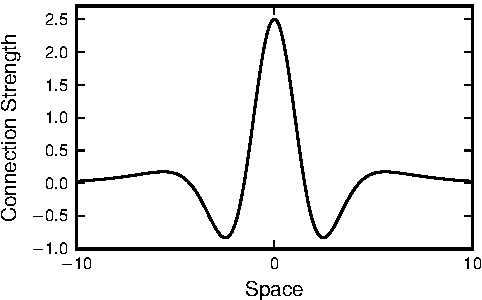
\includegraphics{./Graph/Cross_section_kernel.pdf} 
   	\end{center}
   	\caption{{\bf Mexican-hat connectivity kernel.} The function $w(\cdot)$ is rotationally symmetric (isotropic) about zero, hence a cross-section captures the important aspect of the connectivity kernel's shape. The kernel decays asymptotically to zero.}
 	\label{fig:2d_kernel}
   \end{figure}

\begin{figure}
   	\begin{center}
   		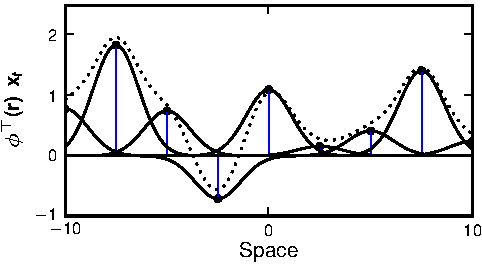
\includegraphics{./Graph/FieldDecomposition.pdf} 
   	\end{center}
   	\caption{{\bf Example of a one-dimensional field decomposition.} A continuous, one-dimensional field decomposed by a finite number of basis functions scaled by the state vector. The dashed line depicts the field, the black solid lines shows the Gaussian basis functions and the vertical lines show the position and amplitude of the states.} 
	\label{fig:FieldDecomposition}
   \end{figure}

 \begin{figure}
    	\begin{center}
     		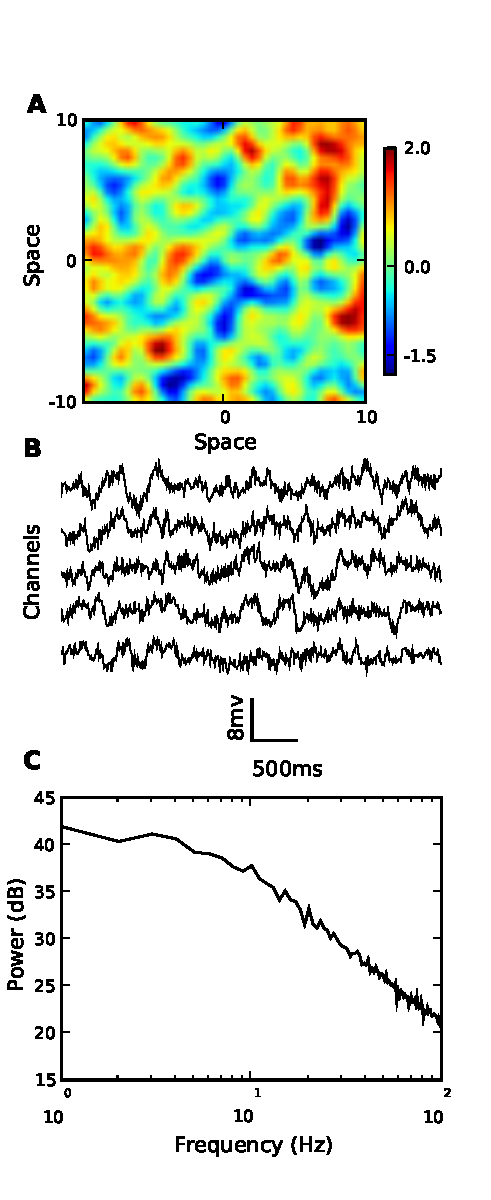
\includegraphics{./Graph/ExperimentalFigure.pdf}
    	\end{center}
    	\caption{{\bf Example of the spatio-temporal properties of the model and synthetically generated data.} \textbf{(A)} The neural field at a single time instant. (\textbf{B}) Data generated by the full neural field model from the first 5 sensors. (\textbf{C}) Power spectral density of the data generated by an observation showing the typical $1/f^2$ characteristic of intracranial EEG.} 
 \label{fig:experimental design}
 \end{figure}

\begin{figure}
\centering
\label{fig:FieldFFT}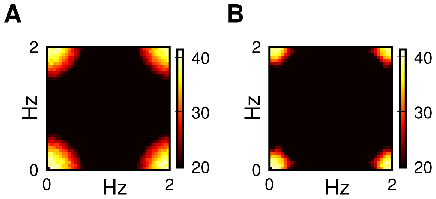
\includegraphics{./Graph/FFTField.pdf}
\caption{{\bf Spatial frequency analysis of the neural field}. (\textbf{A}) The average (over time) power in dB of the spatial frequency of the neural field. (\textbf{B}) The average (over time) power in dB of the spatial frequency of the reconstructed neural field from the basis function decomposition. The reconstructed field shows a narrower bandwidth as a result of the band limiting properties of the sensors and basis functions.}
\label{fig:FFTTrueEstimate}
\end{figure}

\begin{figure*}[!ht] 
	\begin{center}
		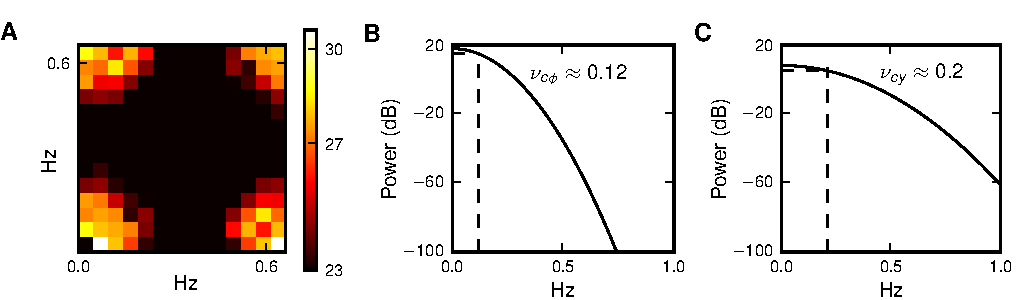
\includegraphics{./Graph/SensorBasisObsFrequencyResponse.pdf}	
	\end{center}
	\caption{{\bf Spatial frequency analysis}. The dashed line shows the cut-off frequency (-3 dB point). (\textbf{A}) The average (over time) power in dB of the spatial frequency of the observations. (\textbf{B}) The spatial frequency response of a one-dimensional model sensor. The symmetry of the sensors and field basis functions allow for the one-dimensional representation of the spectral characteristics. (\textbf{C}) The spatial frequency response of a one-dimensional neural field basis function, illustrating a narrower band width than the sensors. }
	\label{fig:ObservationFreqAnal}
\end{figure*}

\begin{figure}
        \centering
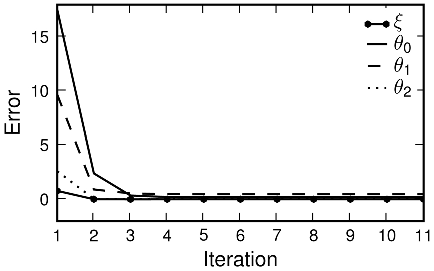
\includegraphics{./Graph/convergence.pdf}
\caption{{\bf Convergence of parameters.} The mean of the absolute error between true and estimated parameters averaged over 100 runs. All parameters converge after six iterations, where the mean difference between errors in consecutive iterations falls below $10^{-4}$.}
\label{fig:ParametersConvergence}
\end{figure}

\begin{figure}
    \centering
    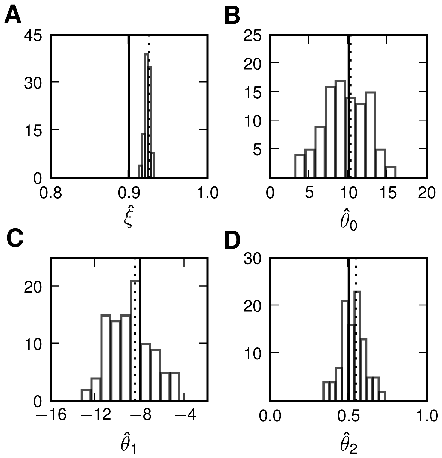
\includegraphics{./Graph/ParametesDistributions.pdf}
  \caption{{\bf Histograms of the parameter estimates over 100
realisations}. The solid lines show the actual values of the parameters and the dotted lines show the means of the estimated parameters. (\textbf{A}) The histogram of the $\xi$ estimates where $\xi=1-\zeta T_s $ and $\zeta$ is the reciprocal of the synaptic time constant. (\textbf{B}) The histogram of the central excitatory connectivity kernel basis function parameter estimates, $\theta_0$. (\textbf{C}) The histogram of the surround inhibition connectivity kernel basis function parameter estimates, $\theta_1$. (\textbf{D}) The histogram of the longer range excitatory connectivity kernel basis function parameter estimates, $\theta_2$.}
\label{fig:Parameters}
\end{figure}

\begin{figure}
    \centering
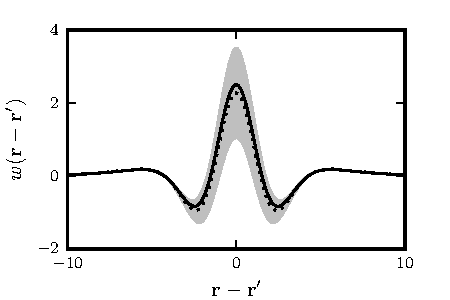
\includegraphics{./Graph/KernelEstimate.pdf}%}
\caption{{\bf Cross-section of connectivity kernel estimate}. The actual kernel is shown by the solid line, the mean kernel estimate (over 100 realisations) is shown by the dotted line and the 95~\% confidence interval is shown by the shaded grey region.}
\label{fig:KernelEstimates}
\end{figure}

  \begin{figure}
   	\begin{center}
   		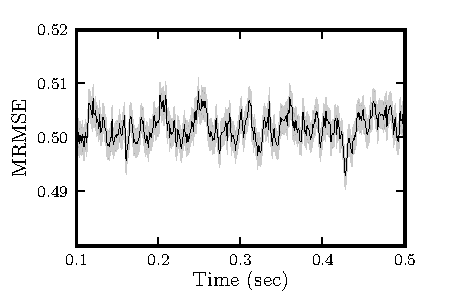
\includegraphics{./Graph/MRMSE.pdf} 
   	\end{center}
   	\caption{{\bf Error in the field reconstruction}. The mean of average RMSE of the estimated field over 100 realisations (solid line) and the 95~\% confidence interval (grey region).} 
\label{fig:RMSE}
   \end{figure}

\begin{figure*}
\centering 
\label{fig:TrueField}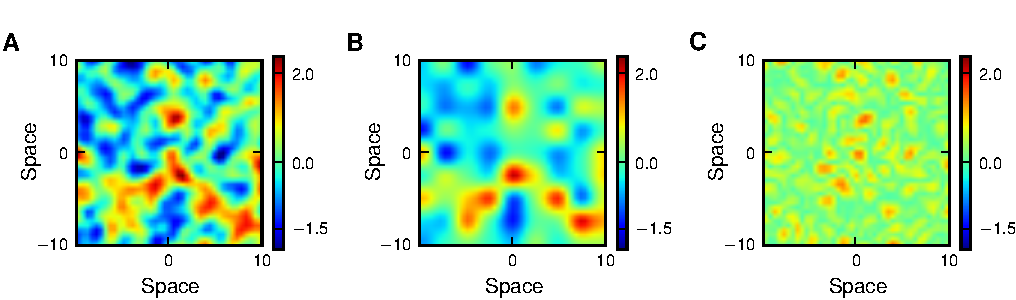
\includegraphics{./Graph/FieldTrueEstimationError.pdf}
\caption{{\bf Examples of the actual and estimated neural fields and the error}. (\textbf{A}) The actual field at a single time instant from the full neural field model that was used to generate the data. (\textbf{B}) The reconstructed field of the reduced model, showing the effect of the basis function decomposition on the frequency content of the estimated field. (\textbf{C}) The absolute error between the true and reconstructed fields. The error shows high frequency behaviour.}
\label{fig:FieldEstimate}
\end{figure*}

\section*{Tables}


\begin{table}[!ht]
\caption{
\bf{Notation}}
\begin{tabular}{|l|l|l|}
	\hline
	\textbf{Symbol} & \textbf{Quantity} & \textbf{Units}\\
	\hline
	\multicolumn{3}{|c|}{\emph{Domain and indices}}\\
	\hline
	$\Omega$ & spatial domain & n.a.\\
	$\mathbf{r}$ & spatial location & [mm, mm]\\
	$t$ & time & s\\
	\hline
	\multicolumn{3}{|c|}{\emph{Model}}\\
	\hline
    $y_t$ & observation & mV\\
    $v(\mathbf{r},t)$ & mean membrane potential & mV \\
	$g(\mathbf{r},t)$ & weighted firing rate function & spikes.s$^{-1}$\\
	$f(\mathbf{r},t)$ & firing rate function & spikes.s$^{-1}$\\
	$e(\mathbf{r},t)$ & field disturbance, with covariance function $\gamma(\mathbf r-\mathbf r')$ & mV\\
	$\boldsymbol\varepsilon_t$ & observation noise, with covariance matrix $\Sigma_\varepsilon$ & mV\\
	$m(\mathbf{r}_n,\mathbf{r}')$ & sensor kernel where $n$ is sensor index $n=1,..,N$ (width $\sigma_m^2$) & n.a. \\
	$w(\mathbf{r},\mathbf{r}')$ & spatial connectivity kernel & n.a.\\
	$h(t)$ & post-synaptic response kernel & mV\\
	$\zeta$, $\xi$ & inverse synaptic time constant \& time constant parameter & s$^{-1}$, n.a.\\
	$\eta(t)$ & Heaviside step function & n.a.\\
	$\delta(t)$ & Dirac-delta function & n.a.\\
	$D$ & temporal differential operator & n.a.\\
	\hline
	\multicolumn{3}{|c|}{\emph{Reduced Model}} \\
	\hline
   	$\boldsymbol\phi(\mathbf{r})$ & vector of $L$ Gaussian basis functions & n.a.\\
   	$\mathbf{x}_t$ & state vector at time $t$ & mV\\
   	$\boldsymbol{\psi}(\mathbf{r}-\mathbf{r}')$ & vector of $n_{\theta}$ connectivity kernel basis functions & n.a.\\
   	$\boldsymbol{\Psi}(\mathbf{r}')$ & decomposition connectivity matrix & n.a.\\
   	$\boldsymbol{\Gamma}$ & inner product of field basis functions & n.a.\\
   	$Q()$ & state transition function & n.a.\\
   	$\mathbf{e}_t$ & state disturbance vector, with covariance $\Sigma_e$ & mV\\
   	$\mathbf{C}$ & observation matrix & n.a. \\
	\hline
	\multicolumn{3}{|c|}{\emph{Frequency Analysis}} \\
	\hline
    % $V(\nu)$ & Fourier transform of the neural field & Hz\\
	$\boldsymbol{\nu}$, $\boldsymbol{\nu}_c$ & spatial frequency and spatial cut-off frequency & Hz \\
	$\sigma_{\nu}^2$ & variance of Fourier transformed Gaussian basis function & Hz$^2$\\
	\hline
	\multicolumn{3}{|c|}{\emph{Estimation}} \\
	\hline
	$\mathcal{X}$ & matrix of sigma vectors & mV\\
	$W$ & matrix of sigma vector weights (scaling parameter $\lambda$) & n.a.\\
   	$\hat{\mathbf{x}}_t^{f-}$, $\hat{\mathbf{x}}_t^f$ & forward prior and posterior state estimates & mV\\
   	$\hat{\mathbf{x}}_t^{b-}$, $\hat{\mathbf{x}}_t^{b}$ & backward prior and posterior state estimates & mV\\
 	$P^{f-}_t$, $P^f_t$  & forward prior and posterior covariance matrices & mV$^2$\\
   	$P^{b-}_t$, $P^b_t$ & backward prior and posterior covariance matrices & mV$^2$\\
	$M_t$& cross-covariance matrix & mV$^2$\\
	$\mathcal K_{t} $ & filter gain & n.a.\\
	$S_t$ & smoother gain & n.a.\\
	$q()$ & nonlinear state function (used in LS estimator) & n.a.\\
   	$\mathcal{\hat{W}}$& vector of parameter estimates (used in LS estimator) & n.a.\\	
	\hline
\end{tabular}
\begin{flushleft}The first column of the table gives the symbols for all the notation used the paper. The second column provides a brief description of the quantity, and the third column provides the SI units where relevant.
\end{flushleft}
\label{tab:Notation}
\end{table}



\renewcommand{\arraystretch}{1.7}
\begin{table}[!ht]
\caption{
\bf{Algorithm for the Unscented RTS Smoother}}
\begin{tabular}{|c|}\hline
\multicolumn{1}{|p{16cm}|}{\textbf{1.} Forward initialisation} \\ 
$\hat{\mathbf x}_0, \mathbf P_0$ \\
\hline
\multicolumn{1}{|p{16cm}|}{\textbf{2.} Forward iteration: for $t \in \left\lbrace 0,\cdots, T\right\rbrace $, calculate the sigma points $\mathcal X_{i,t}^f$ using equations \ref{eq:sigmapoints1}-\ref{eq:sigmapoints3} and propagate through equation~\ref{eq:QmatrixForSigmapoints}} \\
$\mathcal X_{i,t+1}^{f-}=Q(\mathcal X_{i,t}^f) \quad i=0, \dots, 2L$\\
\multicolumn{1}{|p{16cm}|}{Calculate the predicted state and the predicted covariance matrix} \\
$\hat{\mathbf x}_{t+1}^{f-}=\sum_{i=0}^{2L} W_i^{(m)}\mathcal X_{i,t+1}^{f-} $ \\
$\mathbf P_{t +1}^{f-}=\sum_{i=0}^{2L} W_i^{(c)}(\mathcal X_{i,t+1}^{f-}-\hat{\mathbf x}_{t +1}^{f-})(\mathcal X_{i,t+1}^{f-}-\hat{\mathbf x}_{t +1}^{f-})^\top+\boldsymbol \Sigma_e$ \\ 
\multicolumn{1}{|p{16cm}|}{Compute the filter gain, the filtered state and the filtered covariance matrix using the standard Kalman filter update equations} \\
$\mathcal K_{t+1}=\mathbf P_{t +1}^{f-}\mathbf C ^\top(\mathbf C \mathbf P_{t +1}^{f-}\mathbf C ^\top+\boldsymbol \Sigma_{\varepsilon})^{-1}$\\
$\hat{\mathbf x}_{t+1}^{f}=\hat{\mathbf x}_{t+1}^{f-}+\mathcal K_{t+1}(\mathbf y_{t+1}-\mathbf C\hat{\mathbf x}_{t +1}^{f-}) $\\
$\mathbf P_{t+1}^f=(\mathbf I - \mathcal K_{t+1}\mathbf C)\mathbf P_{t +1}^{f-}$\\ 
\hline
\multicolumn{1}{|p{16cm}|}{\textbf{3.} Backward initialisation}\\
$\mathbf P_T^b= \mathbf P_T^f, \quad \hat{\mathbf x}^b_T= \hat{\mathbf x}^f_T$ \\
\hline
\multicolumn{1}{|p{16cm}|}{\textbf{4.} Backward iteration: for $t \in \left\lbrace T-1, \cdots, 0 \right\rbrace $ calculate the sigma points $\mathcal X_{i,t}^b$ and propagate them through equation \ref{eq:QmatrixForSigmapoints}}\\
$\mathcal X_{i,t+1}^{b-}=Q(\mathcal X_{i,t}^b) \quad i=0, \dots, 2L$\\
\multicolumn{1}{|p{16cm}|}{Calculate the predicted state and the predicted covariance matrix}\\
$\hat{\mathbf x}_{t+1}^{b-}=\sum_{i=0}^{2L} W_i^{(m)}\mathcal X_{i,t+1}^{b-}$\\
$\mathbf P_{t +1}^{f-}=\sum_{i=0}^{2L} W_i^{(c)}(\mathcal X_{i,t+1}^{f-}-\hat{\mathbf x}_{t +1}^{f-})(\mathcal X_{i,t+1}^{f-}-\hat{\mathbf x}_{t +1}^{f-})^\top+\boldsymbol \Sigma_e $\\
$\mathbf M_{t +1}=\sum_{i=0}^{2L} W_i^{(c)}(\mathcal X_{i,t}^{b-}-\hat{\mathbf x}_{t}^{f})(\mathcal X_{i,t+1}^{b-}-\hat{\mathbf x}_{t+1}^{b-})^\top$\\
\multicolumn{1}{|p{16cm}|}{Compute the smoother gain, the smoothed state and the smoothed covariance matrix}\\
$\mathbf S_t=\mathbf M_{t +1}\left[ \mathbf P_{t +1}^{b-}\right] ^{-1} $\\
$\hat{\mathbf x}_t^b=\hat{\mathbf x}_t^f+\mathbf S_t\left[\hat{\mathbf x}_{t+1}^{b}-\hat{\mathbf x}_{t+1}^{b-}\right]$\\
$\mathbf P_{t}^{b}=\mathbf P_{t}^{f}+\mathbf S_t\left[\mathbf P_{t+1}^{b}-\mathbf P_{t+1}^{b-} \right]\mathbf S_t^\top $\\
\hline
\end{tabular}
\begin{flushleft}This table shows the steps in the unscented Rauch-Tung-Striebel smoother algorithm. The steps are iterated 11 times for our state estimation procedure. The least squares algorithm is run after each iteration to update the parameter estimates.
\end{flushleft}
\label{tab:UKFAlgorithm}
\end{table}
\renewcommand{\arraystretch}{1}

\begin{table}[!ht]
\caption{
\bf{Parameters}}
\begin{tabular}{|c|l|c|l|}
	\hline
	\textbf{Symbol} & \textbf{Quantity} & \textbf{Value} & \textbf{Units}\\
	\hline
	\multicolumn{4}{|c|}{\emph{Domain and indices}}\\
	\hline
	$\Delta$ & spatial discretisation step & 0.5 & mm \\
	$T_s$ & time step & $0.001$ & s\\
	$T$ & number of time steps used in estimation & 0.4 & s\\
	\hline 
\multicolumn{4}{|c|}{\emph{Model}}\\
	\hline
	$\tau$ & synaptic time constant & 0.01 & s$^{-1}$ \\
	$f_{max}$ & maximal firing rate & 10 & spikes.s$^{-1}$\\
	$\varsigma$ & slope of sigmoidal activation function & 0.8 & mV$^{-1}$\\
	$v_0$ & firing threshold & 2 & mV \\
	$\boldsymbol{\theta}$ & vector of connectivity kernel parameters & $\left[\begin{array}{ccc}
	10 &-8 &0.5
	\end{array}
	\right]^{\top}$ & mV.spike$^{-1}$\\
	$\sigma_{\psi_{1}}, \sigma_{\psi_{2}}, \sigma_{\psi_{3}}$ & connectivity kernel width parameters & 1.8, 2.4, 6 & mm\\
	$N$ & number of sensors & 196 & n.a.\\ 
	$\Delta_y$ & distance between adjacent sensors & 1.5 & mm\\
	$\sigma_{m}$ & sensor width parameter & 0.9 & mm \\
	$\Sigma_{\varepsilon}$ & observation noise variance & $0.1 \times I_{N}$ & mm$^2$ \\
	$\sigma_{\gamma}$& disturbance spatial covariance width & 1.3 & mm\\
	$\sigma_{\gamma,t}$ & disturbance temporal variance & 0.1 & mV \\
	\hline 
	\multicolumn{4}{|c|}{\emph{Reduced Model}}\\
	\hline
	$L$ & number of basis functions& 81 & n.a.\\
	$\Delta_{\phi}$ & distance between field basis functions & 2.5 & mm \\
	$\sigma^2_{\phi}$ & Spatial variance of Gaussian in spatial domain & 2.5 & mm$^2$\\
	\hline 
	\multicolumn{4}{|c|}{\emph{Frequency Analysis}}\\
	\hline
	$\rho_y$ & sensor over-sampling parameter & 1 & n.a.\\
	$\rho_\phi$ & field basis function over-sampling parameter & 1 & n.a.\\
	\hline 
	\multicolumn{4}{|c|}{\emph{Estimation}}\\
	\hline
	$\alpha$& determines the spread of sigma points & 0.001 & n.a.\\
	$\beta$& prior knowledge of the sigma points distribution & 2 & n.a.\\
	$\kappa$& scaling parameter $(3-L)$& -78 & n.a.\\
	$\lambda$& scaling parameter & -80.99 & n.a.\\
	\hline
\end{tabular}
\begin{flushleft}Parameters for the neural field model, the model reduction, the frequency analysis and the estimation procedure.
\end{flushleft}
\label{tab:Parameters}
\end{table}
	

\begin{table}[!ht]
\caption{
\bf{Estimation Results}}
\begin{tabular}{|p{1.5cm}|p{1.5cm}|p{2.5cm}|p{1.5cm}|}
		
\hline
Parameter & Actual Value & Mean Estimate $\pm$ Std. Dev. & Bias (\%) \\
\hline
$\xi$ & $0.9$ & $0.925\pm 0.004$ & $2.778$ \\
$\theta_0$ & $10$ & $10.228\pm2.794$ & $2.28$\\
$\theta_1$ & $-8$ & $-8.495\pm1.913$ & $-6.187$\\
$\theta_2$ & $0.5$ & $0.545\pm0.077$ & $9$\\
\hline
\end{tabular}
\begin{flushleft}Actual parameter values compared to mean parameter estimates obtained from the 100 Monte Carlo simulations.
\end{flushleft}
\label{tab:Parameters estimates}
\end{table}

\end{document}

